\section{Actividad No 03 – Herramientas Similares al GitHub} 
		
\begin{itemize} % CREA GUIONES
\item \textbf{¿Que es GitHub?}\\

GitHub es un servicio de alojamiento web para proyectos que utilizan el sistema de control de revisiones Pequeño icono de GitGit . Está escrito en Ruby on Rails por los desarrolladores de Logical Awesome Chris Wanstrath, PJ Hyett y Tom Preston-Werner. GitHub ofrece planes comerciales y cuentas gratuitas para proyectos de código abierto.

El sitio proporciona funciones de redes sociales como una alimentacion de contenido, seguidores y el gráfico de red para mostrar cómo los desarrolladores trabajan en sus versiones de un repositorio.

Otros autores lo señalan como una plataforma de desarrollo colaborativo de software para alojar proyectos utilizando el sistema de control de versiones Git,debido a que el código se almacena de forma pública, aunque también se puede hacer de forma privada, creando una cuenta de pago.\\

\begin{center}

\includegraphics[width=6cm]{./Imagenes/actividad0301} 
\end{center}
	
\end{itemize} 


\begin{itemize} % CREA GUIONES
\item \textbf{¿Porque es importante GitHub?}\\

GitHub permite alojar en tu repositorio el código de desarrollo de proyecto y te brinda herramientas muy útiles para el trabajo en equipo, dentro de un proyecto.

Además de eso, puedes contribuir a mejorar el software de los demás. Para poder alcanzar esta meta, GitHub provee de funcionalidades para hacer un fork y solicitar pulls.

Realizar un fork es simplemente clonar un repositorio ajeno (genera una copia en tu cuenta), para eliminar algún bug o modificar cosas de él. Una vez realizadas tus modificaciones puedes enviar un pull al dueño del proyecto. Éste podrá analizar los cambios que has realizado fácilmente, y si considera interesante tu contribución, adjuntarlo con el repositorio original.\\

\begin{center}
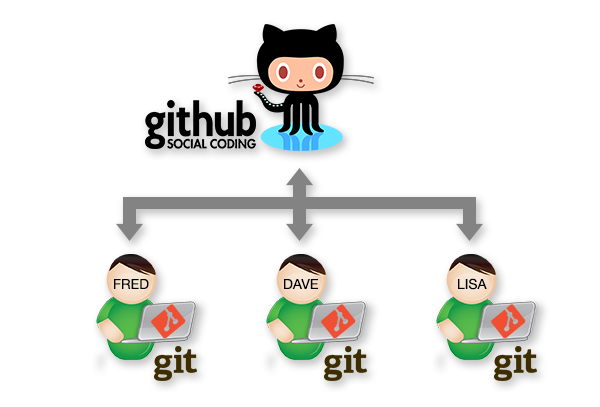
\includegraphics[width=12cm]{./Imagenes/actividad0302} 
\end{center}
	
\end{itemize} 


\begin{itemize} % CREA GUIONES
\item \textbf{¿Qué herramientas proporciona?}\\

En la actualidad, GitHub es mucho más que un servicio de alojamiento de código. Además de éste, se ofrecen varias herramientas útiles para el trabajo en equipo. Entre ellas, caben destacar:

\begin{enumerate}[1.]

\item Una wiki para el mantenimiento de las distintas versiones de las páginas.\\

\item Un sistema de seguimiento de problemas que permiten a los miembros de tu equipo detallar un problema con tu software o una sugerencia que deseen hacer.\\

\item Una herramienta de revisión de código, donde se pueden añadir anotaciones en cualquier punto de un fichero y debatir sobre determinados cambios realizados en un commit específico.\\

\item Un visor de ramas donde se pueden comparar los progresos realizados en las distintas ramas de nuestro repositorio.\\

\end{enumerate}	
\end{itemize} 

\begin{itemize} % CREA GUIONES
\item \textbf{Herramientas Similares al GitHub}\\

A pesar de que GitHub sea la plataforma más utilizada para almacenar proyectos basados en código abierto en Internet, existen otras opciones que se puede elegir para publicar y almacenar en la nube nuestros proyectos,entre los cuales tenemos:

\begin{enumerate}[1.]

\item Bitbucket\\

Bitbucket se trata de otra plataforma muy popular en la que individuos y organizaciones tienden a almacenar sus repositorios basados en código libre. 

Permite tener repositorios públicos, como así también privados ilimitados, lo cual atrae la atención de los desarrolladores que acostumbran a necesitar espacio de almacenamiento para almacenar sus archivos en la nube.

\begin{center}
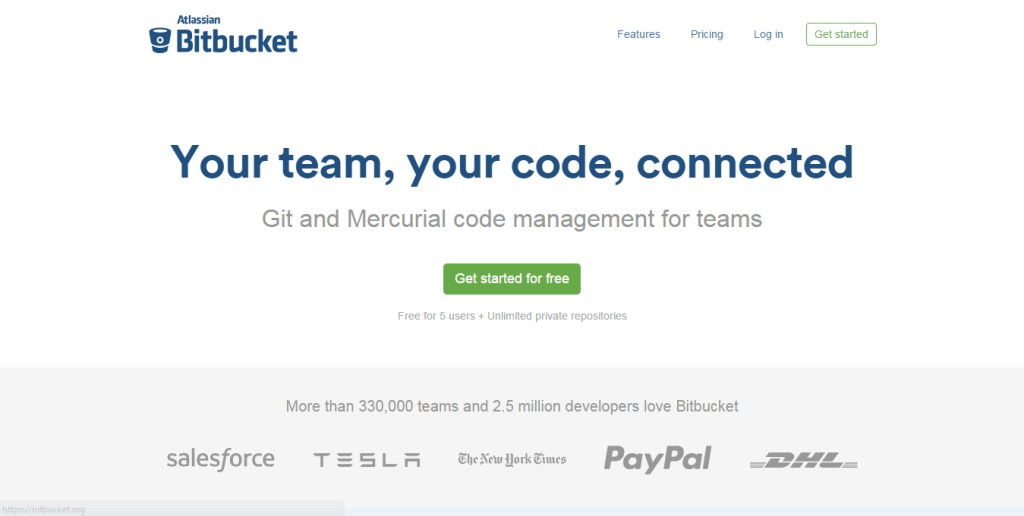
\includegraphics[width=12cm]{./Imagenes/actividad0303} 
\end{center}

\item SourceForge\\

SourceForge es otra reconocida página web en el que desarrolladores acostumbran a publicar sus proyectos basados en diferentes plataformas y compatibles con los más variados sistemas operativos, como Linux, Windows y Mac. 

Una de las particularidades de SourceForge es que permite únicamente crear proyectos de código abierto con nombre único, por lo que deberemos ser originales al momento de publicar nuestras creaciones. 

\begin{center}
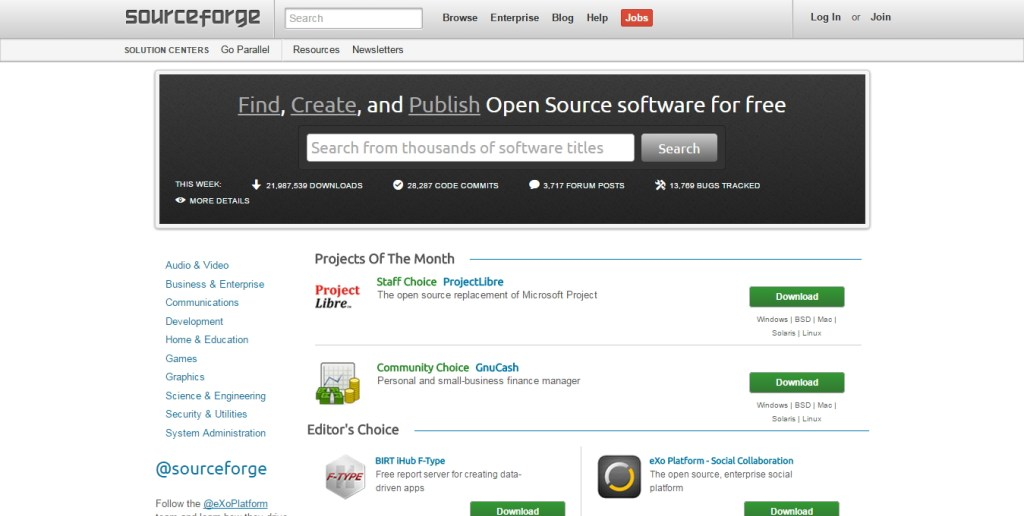
\includegraphics[width=12cm]{./Imagenes/actividad0304} 
\end{center}

\item GitLab\\

GitLab es una página web similar, aunque en este caso destaca la posibilidad de permitirle a sus usuarios instalar esta plataforma en sus servidores particulares, lo cual permite no tan solo que el usuario pueda asociar un dominio personal a su cuenta de GitLab, sino que también puede asociar un servidor web propio, lo cual le permitirá gozar de mayor seguridad y privacidad en los contenidos.

\begin{center}
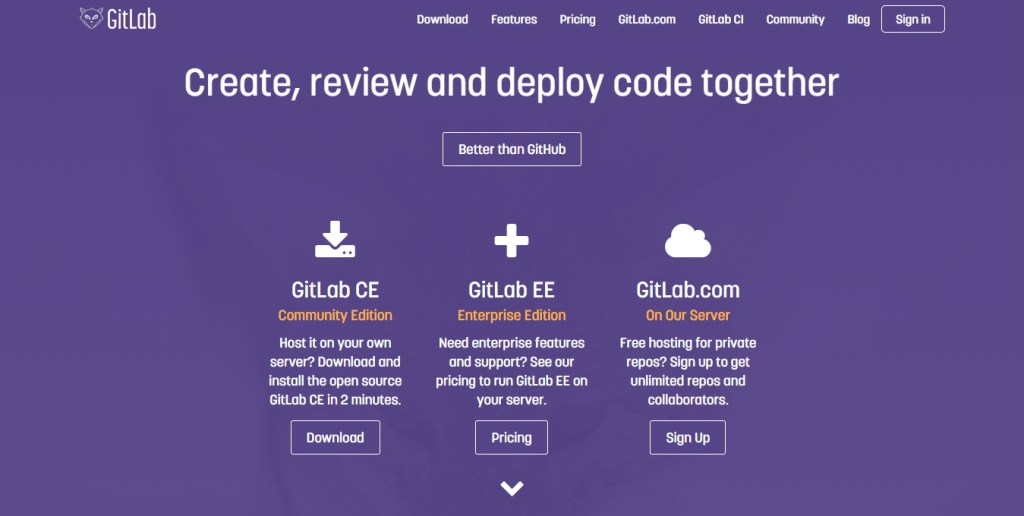
\includegraphics[width=12cm]{./Imagenes/actividad0305} 
\end{center}

\item Kiln\\

El host Kiln es una opción de pago que ofrece mejores servicios. 
Al contratar un plan dentro de este host conseguiremos obtener de manera gratuita un subdominio para nuestra empresa, desde el cual podremos almacenar todos nuestros proyectos en una página web particular.

\begin{center}
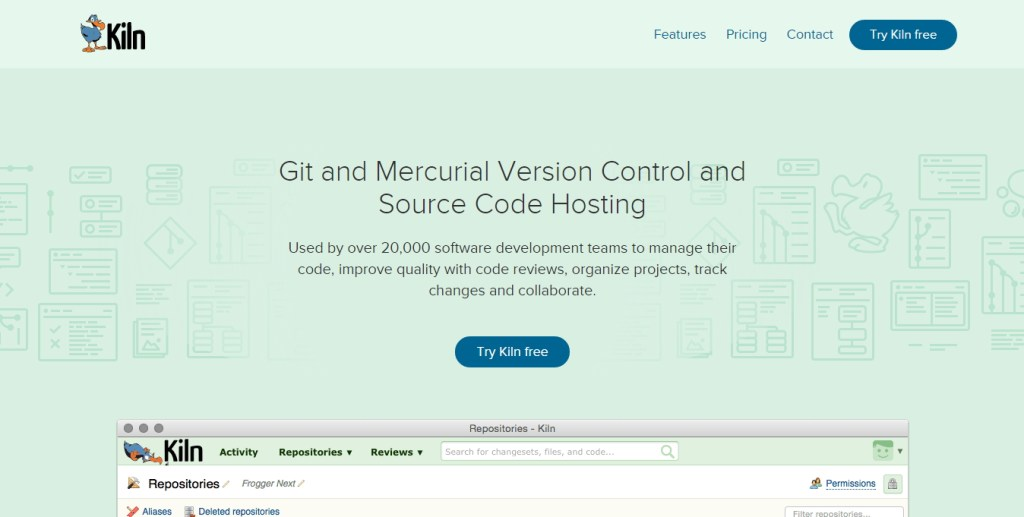
\includegraphics[width=12cm]{./Imagenes/actividad0306} 
\end{center}

\item Codeplane\\

Codeplane es otro servicio de pago, a través del cual podremos almacenar nuestros proyectos en Internet. 
También dentro de este servicio tenemos herramientas como es el caso de la copia de seguridad de los repositorios, y las posibilidades de publicación de proyectos.

\begin{center}
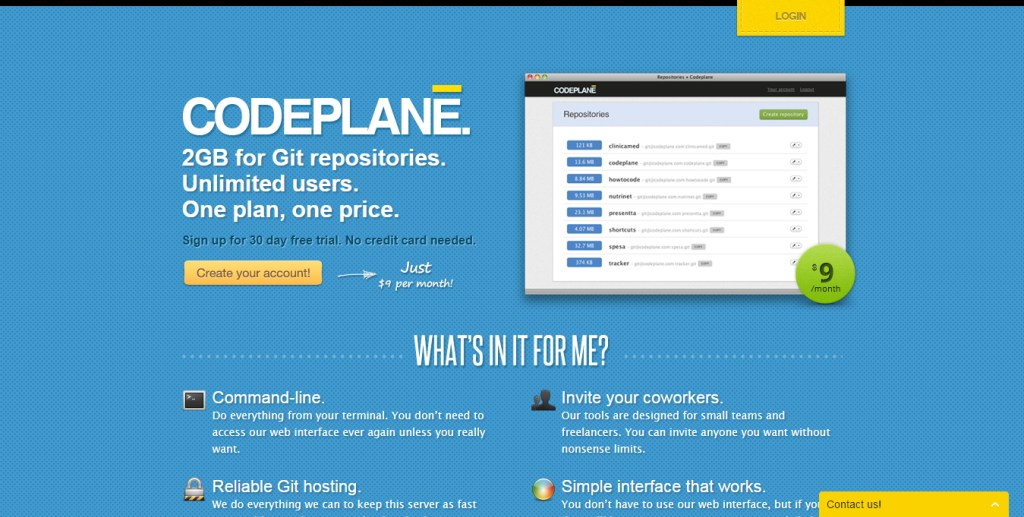
\includegraphics[width=12cm]{./Imagenes/actividad0307} 
\end{center}

\item CodePlex\\

Microsoft nos ofrece un servicio gratuito de almacenamiento de código fuente llamado CodePlex, el cual nos permite crear proyectos e incluso tener nuestro propio sitio con subdominio.

Para publicar proyectos necesitaremos hacerlo con títulos únicos, ya que al igual que SourceForge, CodePlex no nos permite realizar publicaciones con el mismo nombre para buscar originalidad en los proyectos.

\begin{center}
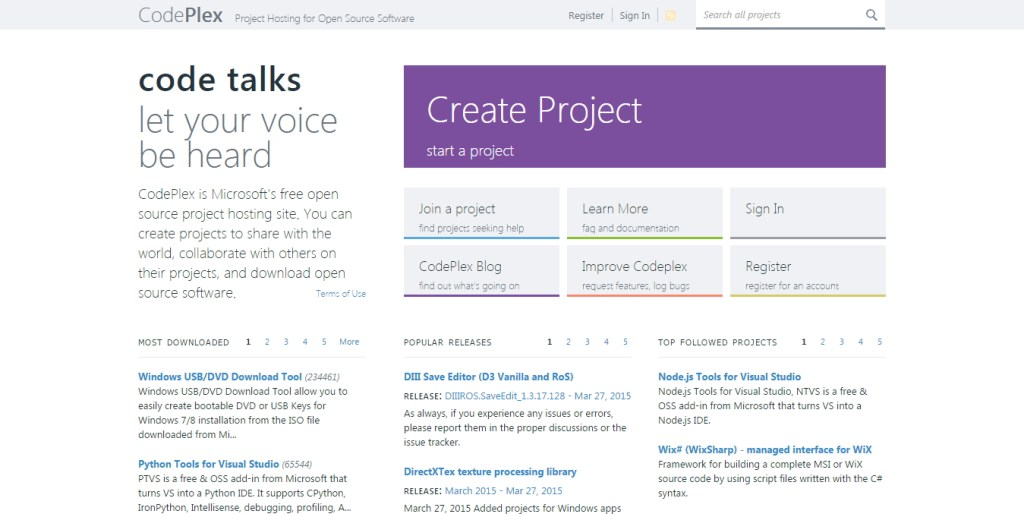
\includegraphics[width=12cm]{./Imagenes/actividad0308} 
\end{center}

\item Beanstalk\\

Beanstalk es una plataforma premium que nos ofrece cuentas gratuitas por dos semanas para probar el alcance de cada función que incluye. No necesitaremos herramientas adicionales, ya que al igual que GitHub, podremos editar el código desde nuestro navegador web.

\begin{center}
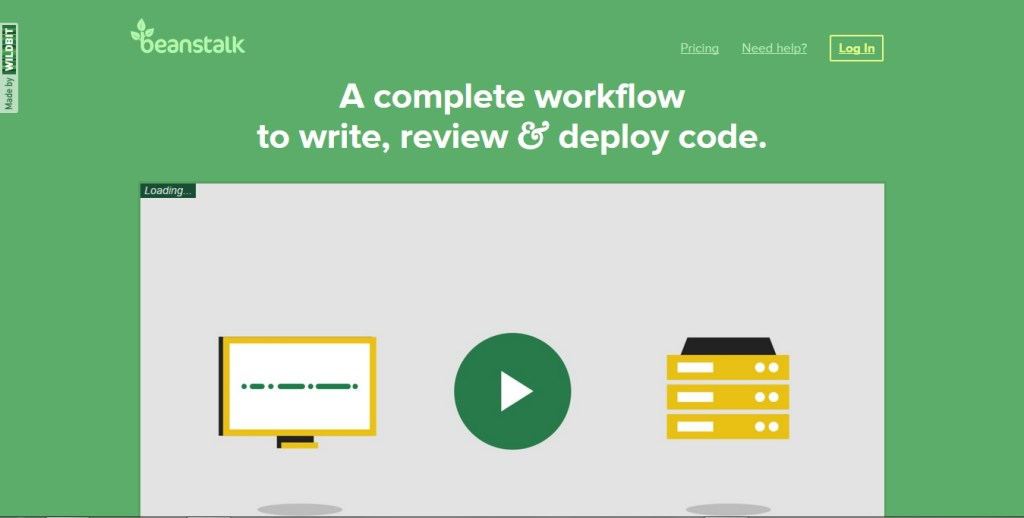
\includegraphics[width=12cm]{./Imagenes/actividad0309} 
\end{center}

\end{enumerate}

\end{itemize} 




